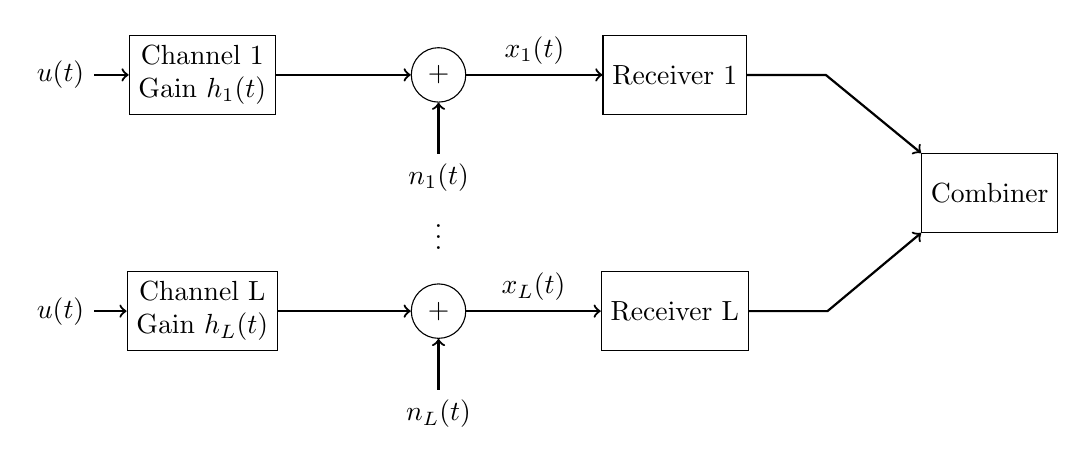
\begin{tikzpicture}
    \node (u1) {$u(t)$};
    \node[below of=u1, node distance=3cm] (uL) {$u(t)$};
    
    \path (u1) -- (uL) node[midway] (middle) {};
    
    \node[right of=u1, draw, minimum width=1.2cm, minimum height=1cm, node distance=1.8cm,align=center] (c1) {Channel 1\\Gain $h_1(t)$};
    \node[right of=c1, draw, circle, node distance=3cm] (p1) {$+$};
    \node[right of=p1, draw, minimum width=1.2cm, minimum height=1cm, node distance=3cm] (r1) {Receiver 1};
    \draw[->, thick] (u1) -- (c1);
    \draw[->, thick] (c1) -- (p1);
    \draw[->, thick] (p1) -- (r1) node[above,midway] {$x_1(t)$};
    \draw[<-, thick] (p1) -- ++(0,-1) node[below] {$n_1(t)$};
    
    \node[right of=uL, draw, minimum width=1.2cm, minimum height=1cm, node distance=1.8cm,align=center] (cL) {Channel L\\Gain $h_L(t)$};
    \node[right of=cL, draw, circle, node distance=3cm] (pL) {$+$};
    \node[right of=pL, draw, minimum width=1.2cm, minimum height=1cm, node distance=3cm] (rL) {Receiver L};
    \draw[->, thick] (uL) -- (cL);
    \draw[->, thick] (cL) -- (pL);
    \draw[->, thick] (pL) -- (rL) node[above,midway] {$x_L(t)$};
    \draw[<-, thick] (pL) -- ++(0,-1) node[below] {$n_L(t)$};
    
    \path (r1) -- ++(4,0) coordinate (NE);
    
    \node[draw, minimum width=1.2cm, minimum height=1cm, node distance=2cm] (comb) at (NE |- middle) {Combiner};
    
    \draw[->, thick] (r1.east) -- ++(1,0) -- (comb.north west);
    \draw[->, thick] (rL.east) -- ++(1,0) -- (comb.south west);
    
    \path (p1) -- (pL) node[pos=.7] {$\vdots$};
    
\end{tikzpicture}